% This is samplepaper.tex, a sample chapter demonstrating the
% LLNCS macro package for Springer Computer Science proceedings;
% Version 2.20 of 2017/10/04
%
\documentclass[runningheads]{llncs}
%
\usepackage{graphicx}
% Used for displaying a sample figure. If possible, figure files should
% be included in EPS format.
%
% If you use the hyperref package, please uncomment the following line
% to display URLs in blue roman font according to Springer's eBook style:
% \renewcommand\UrlFont{\color{blue}\rmfamily}

\begin{document}
%
\title{Cell Based Analysis for Mouse Brain Images\thanks{Supported by organization x.}}
%
%\titlerunning{Abbreviated paper title}
% If the paper title is too long for the running head, you can set
% an abbreviated paper title here
%
\author{Kui Qian\inst{1}\orcidID{0000-1111-2222-3333} \and
Yoav Freund\inst{2}\orcidID{1111-2222-3333-4444} }
%
\authorrunning{F. Author et al.}
% First names are abbreviated in the running head.
% If there are more than two authors, 'et al.' is used.
%
\institute{Department of Electrical and Computer Engineering, University of California San Diego, La Jolla CA 92093, USA \and
Department of Computer Science and Engineering, University of California San Diego, La Jolla CA 92093, USA \\\email{yfreund@eng.ucsd.edu}
}
%
\maketitle              % typeset the header of the contribution
%
\begin{abstract}
The abstract should briefly summarize the contents of the paper in
150--250 words.

\keywords{First keyword  \and Second keyword \and Another keyword.}
\end{abstract}
%
%
%
\section{Introduction}


\section{Method}
\subsection{Extraction of Cell Shape Features}


\subsection{Mouse Brain Alignment Using Landmarks}


\subsection{Statistically Significant Regions}

Landmarks are chosen by anatomists, which are typically biologically significant groups of neurons. Because cell shape feature extraction is under an unsupervised way, our method can suggest landmarks by detecting brain regions whose cytoarchitecture is significantly different from the average.

\subsubsection{Statistical Significance of Patches}

We compare regions by using the Kolmogorov-Smirnov (KS) test to discriminate CDFs of cell shape features. Specifically, we define KS significance by sorting the features based on decreasing KS values. The score is then defined as the sum of the M most significant features,
\begin{equation}
score=\sum_{i=1}^{M}{-\log{KS(x_i, B_i)}}
\end{equation}
where $x_i$ and $B_i$ are the CDFs of the $i$th feature of the patch and the contrast region respectively.

The image is divided into overlapping windows with a size of 100 microns and a stride of 50 microns. Images of 5 consecutive sections are included together to expand 2D patches to 3D cubes. 


\subsubsection{Heuristics for Finding Significant Regions}

The following process is done sequentially, each iteration generating one significant region. The whole images are viewed as background while the significant regions are viewed as foreground. We repeat this process N times to generate N significant regions.
\begin{enumerate}
  \item Find the cube (100 microns cubed) with the highest KS significance compared to the background.
  \item Expand the cube to a region according the following rules:
  		\begin{itemize}
 			 \item Starting from the chosen cube, slide a window in all directions by a stride of half window size and then select the 8 closest cubes around to judge as background or foreground.
  			 \item For the new foreground cubes, use the same way till no new ones appear.
 			 \item A cube is recognized as foreground if $dist(x,S_B )>\alpha \cdot dist(x,S_F)$ where $S_F$ represents the CDFs of cells in the most significant cube and $S_B$ represents the CDFs of cells in the background. $\alpha$ is set to be 3.
		\end{itemize}
\end{enumerate}

\begin{figure}
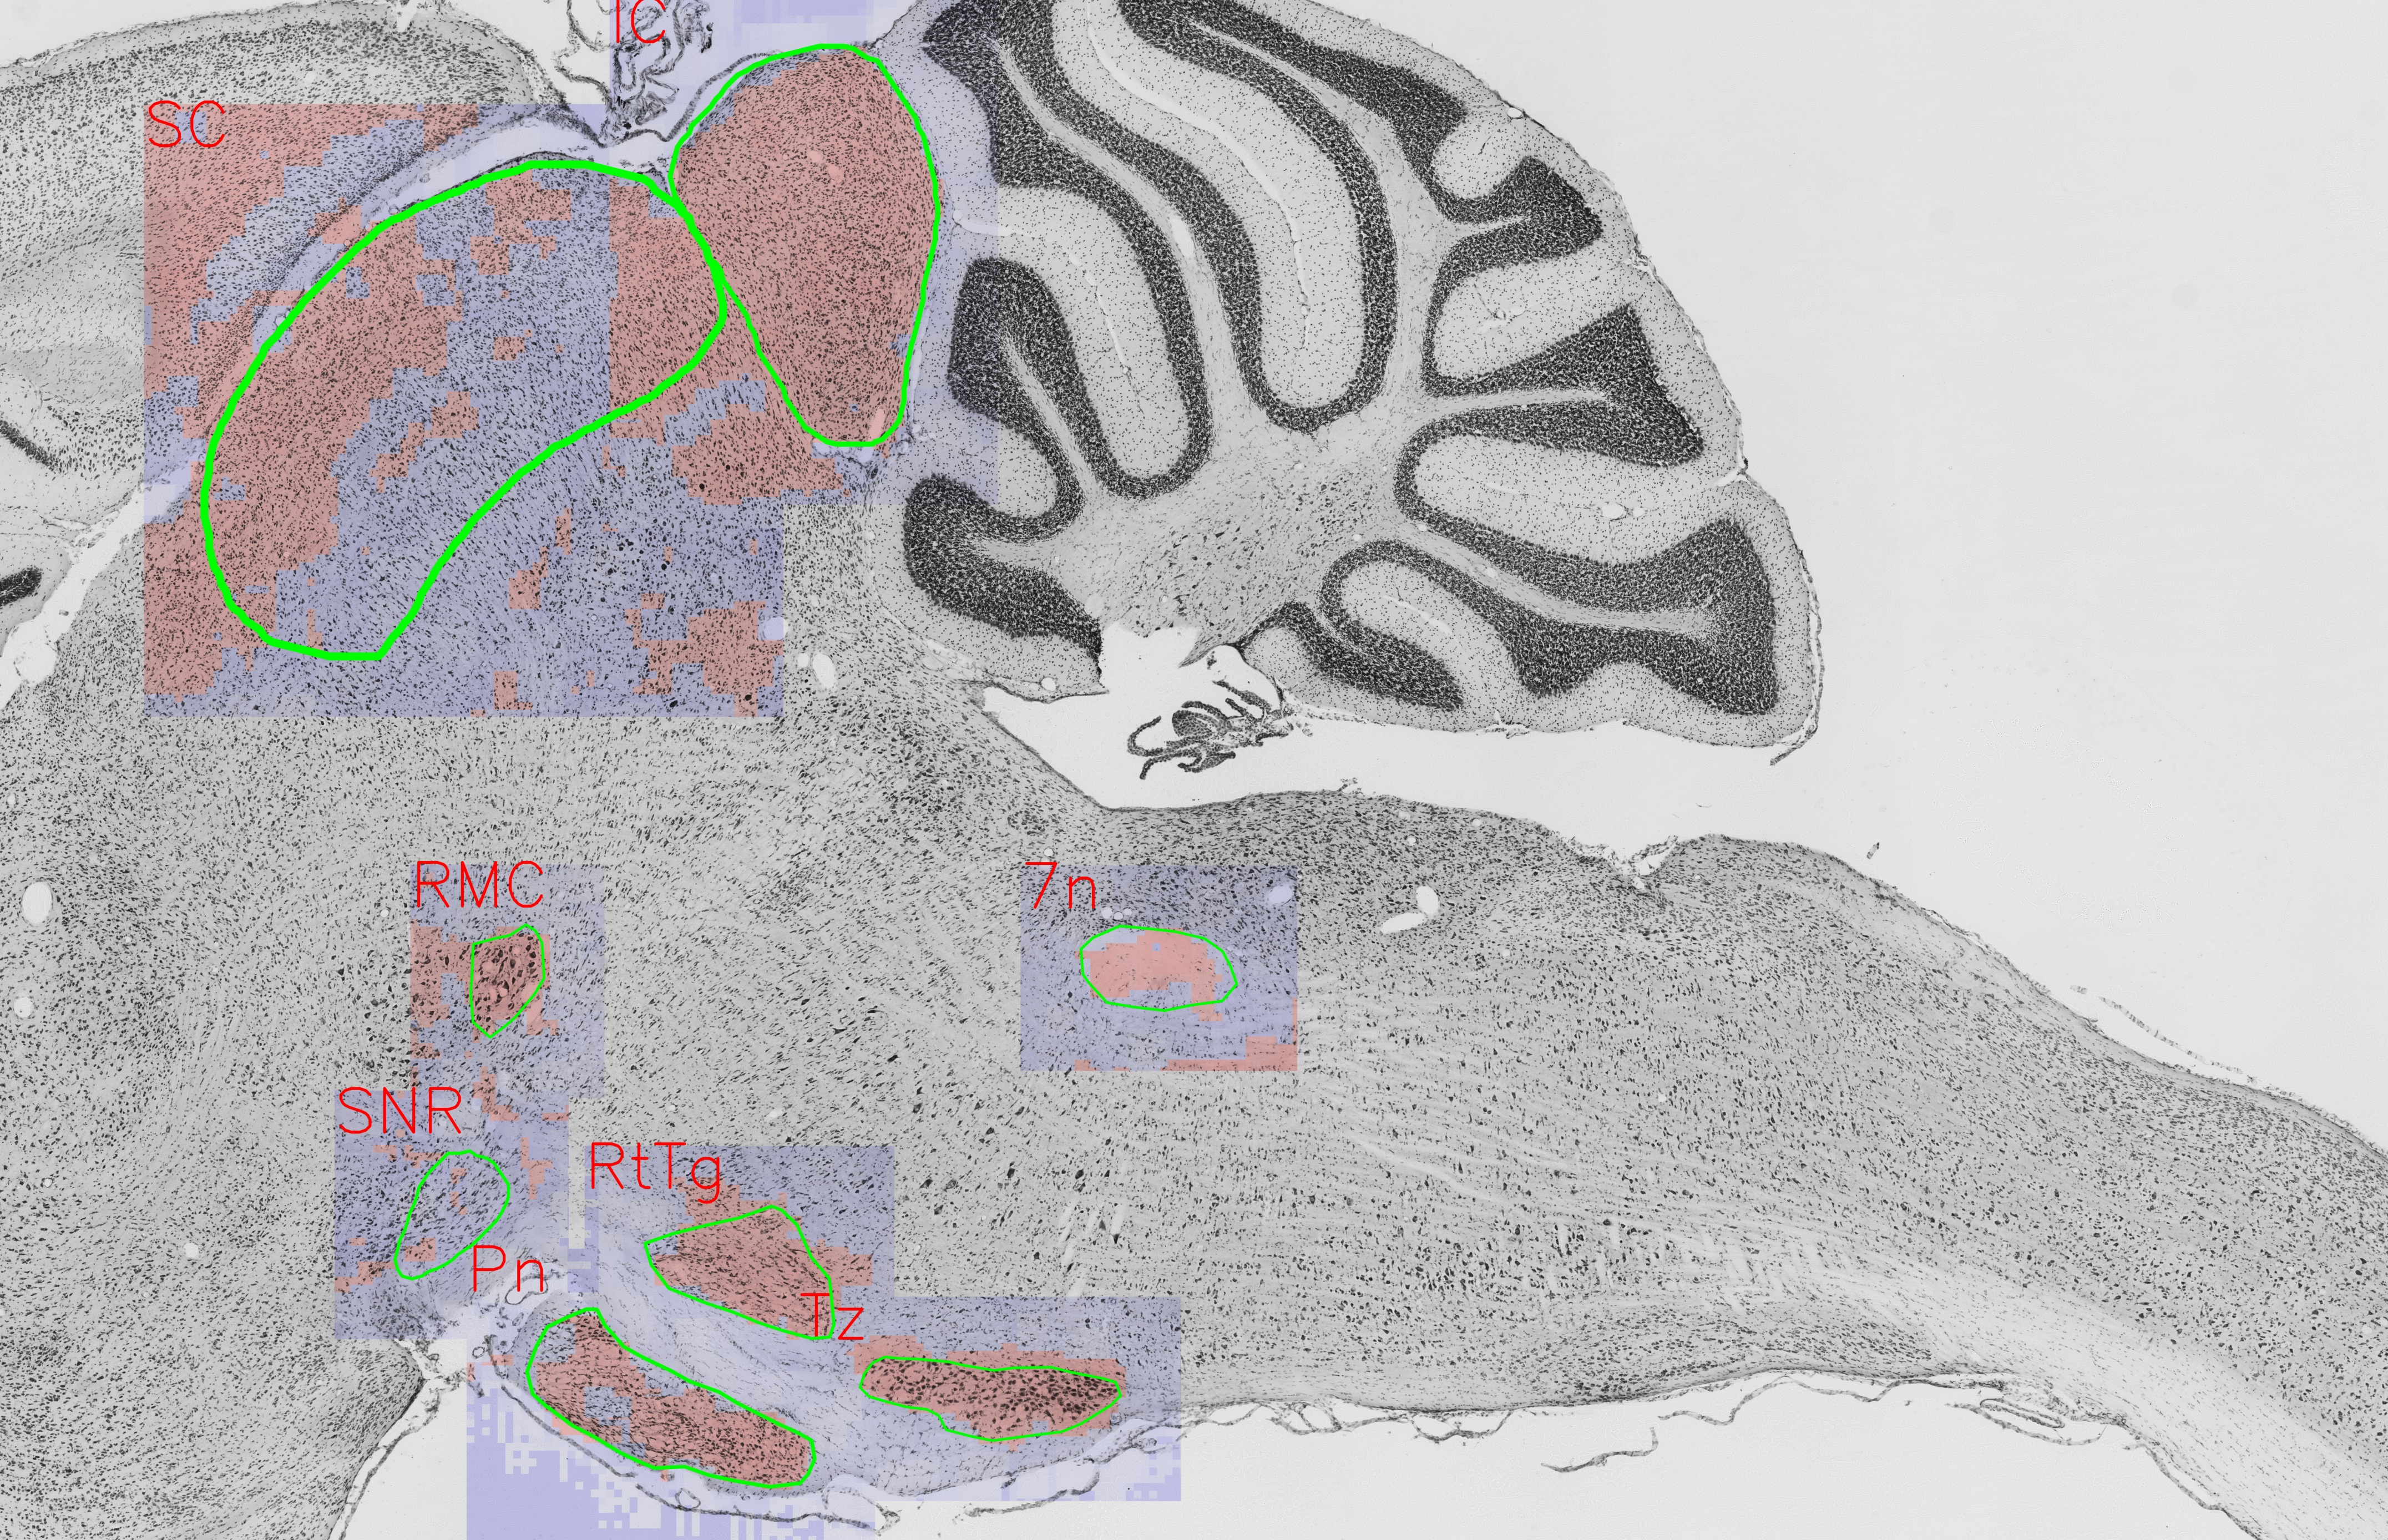
\includegraphics[width=\textwidth]{256.png}
\caption{One example detection score map of mouse brain sections. For one brain structure, patches in its local region are labeled as red when their detection scores are positive and blue otherwise. Green contours are annotations of structures by anatomists.}
\label{scoremap}
\end{figure}

\section{Experiments and Results}


\subsection{Detection Score Map}

\subsection{Detection Score Accuracy Based on Landmark Shifts}



\begin{figure}
\includegraphics[width=\textwidth]{shift1.jpg}
\caption{Detection scores as function of translation in one direction among X, Y and Z. 10 mouse brain structures are included.}
\label{1Dshift}
\end{figure}


\begin{figure}
\includegraphics[width=\textwidth]{Shift3D.png}
\caption{Detection scores as function of translation in three planes for one structure, Lateral reticular nucleus (LRt). Intersection points of two red dashed lines are the locations of maximum and red contours mark half the maximum. The three images at the bottom are local regions of LRt taken from three mouse brain sections. Green contours are annotations by anatomists.}
\label{3Dshift}
\end{figure}


\begin{figure}
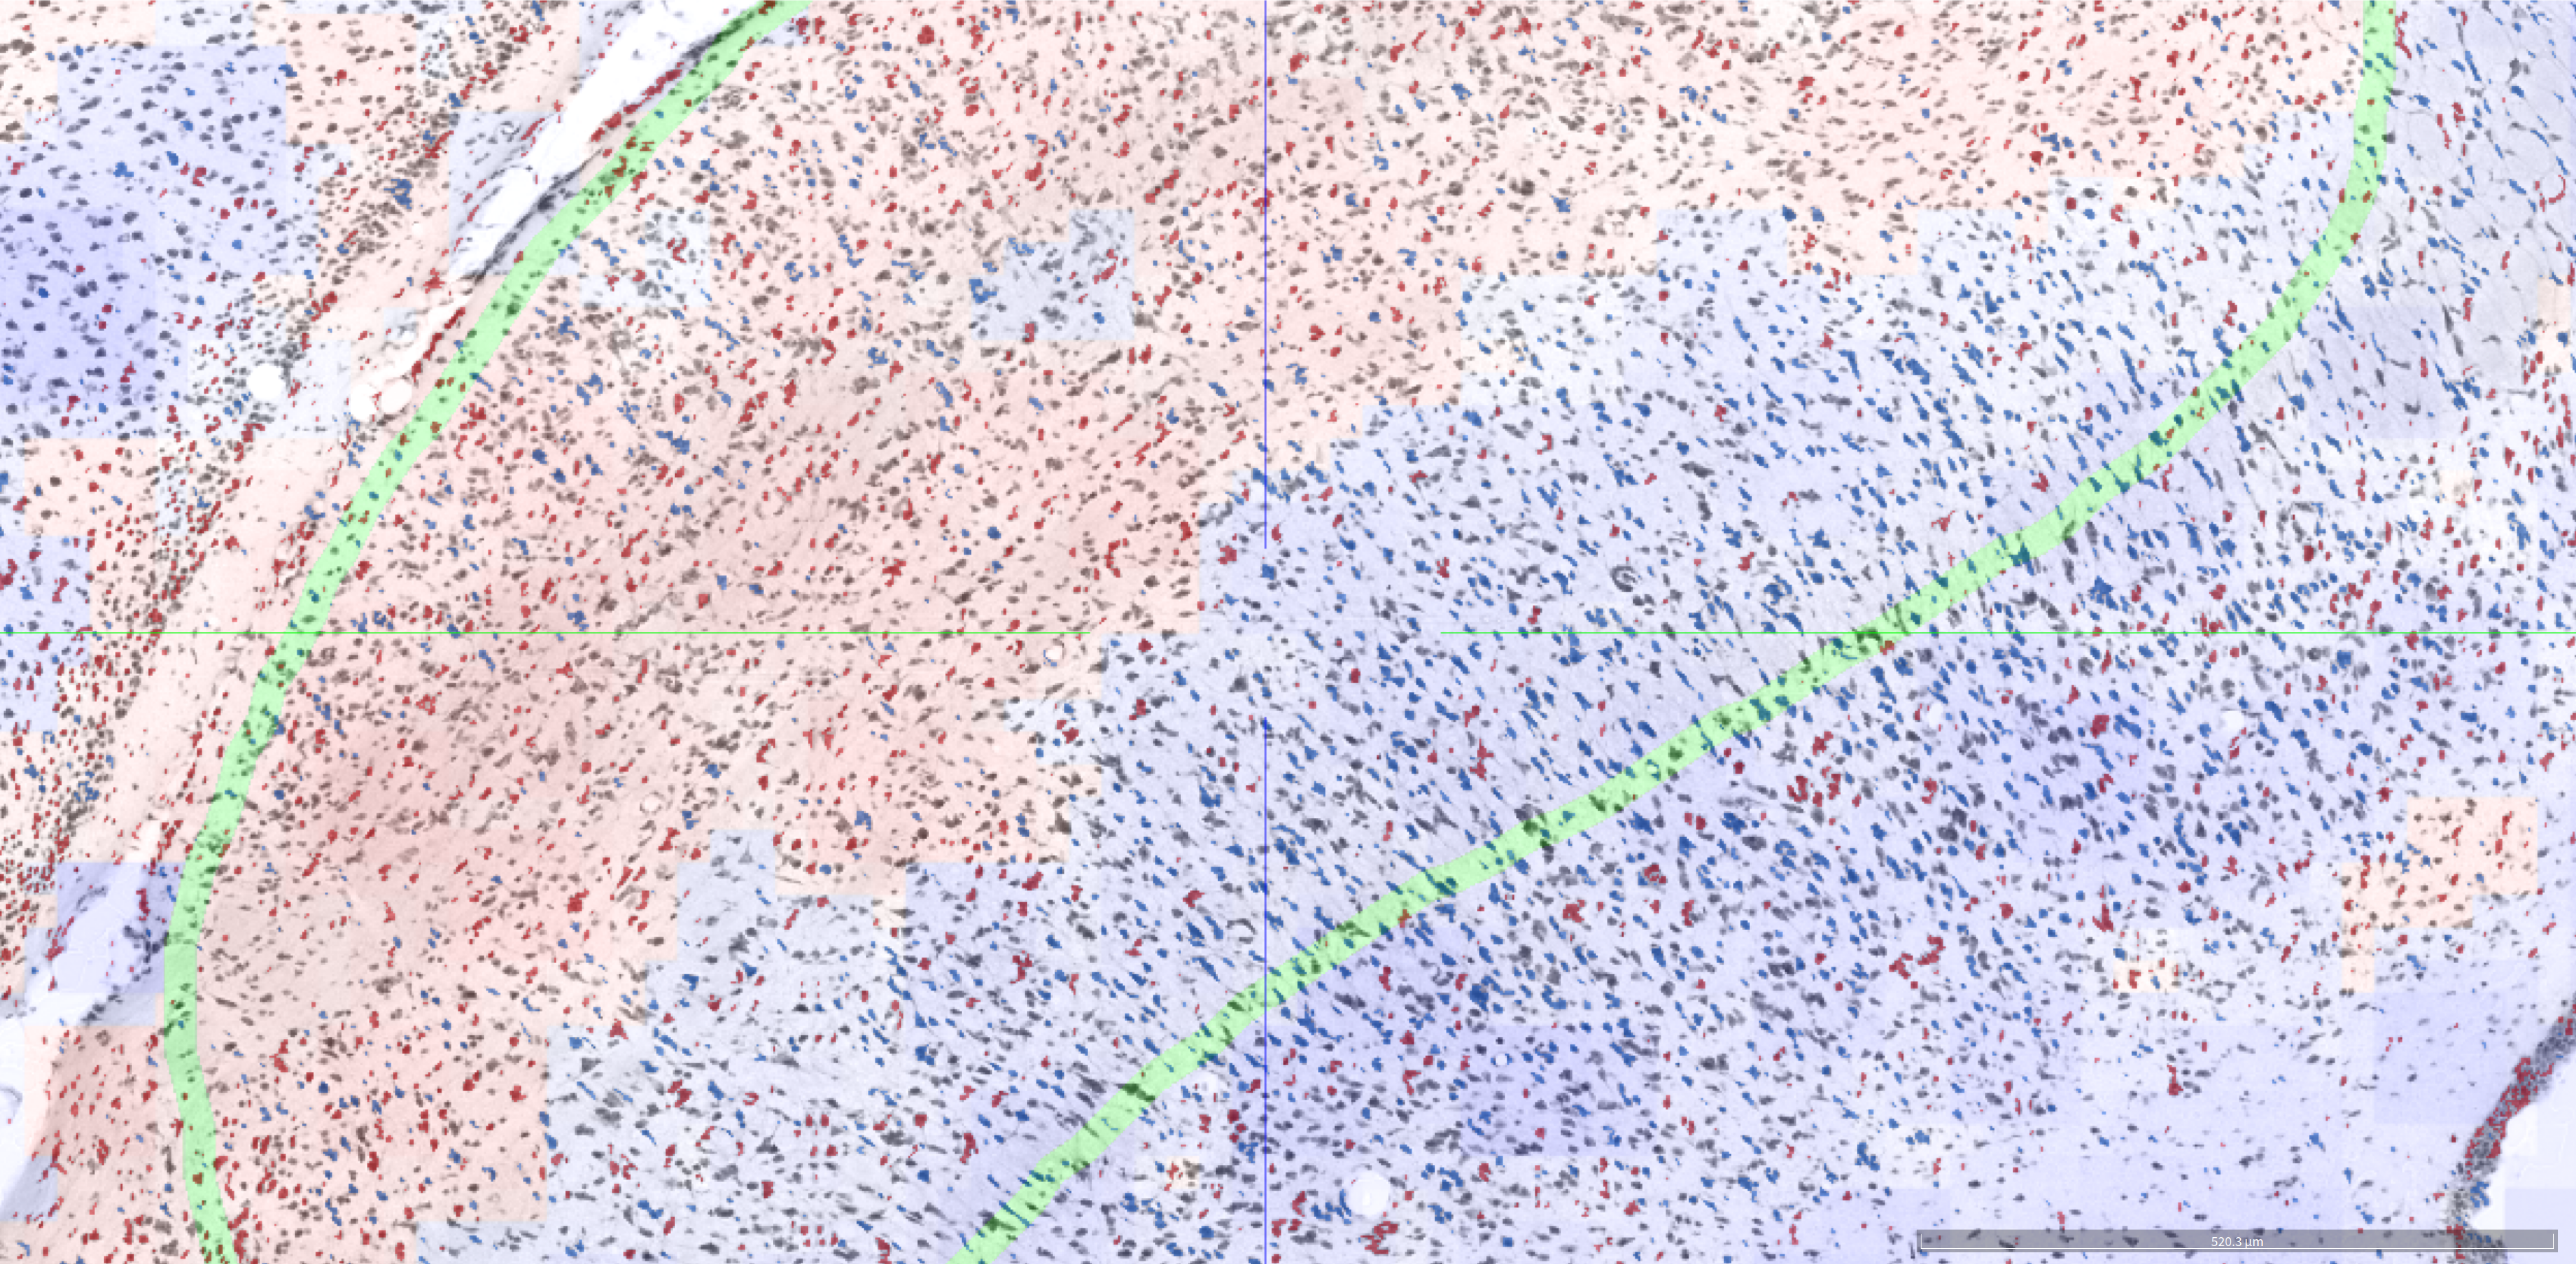
\includegraphics[width=\textwidth]{Screenshot.png}
\caption{One example of visualizing features' function in detection. The image shows a region of a mouse brain structure, superior colliculus (SC). Patches are labeled as red when their detection scores are positive and blue otherwise. Red cells are those with rotation values ranging from 20 to 60 while blue ones are those with rotation values ranging from -50 to 10. Green contours are annotations by anatomists. The visualization software is WebKnossos.}
\label{webknossos}
\end{figure}


\subsection{Visual Feedback of Detection}

Usually the detected region for a structure is larger or smaller than the contour marked by anatomists. To help anatomists determine whose results are better between the detector and themselves, we give them feedback showing how the detector works. Because cells are anatomical units and elements of feature vectors as input of the detector are CDFs of cell shape features, the feature importance values returned by the XgBoost Classifier directly show which shape features the detector cares. Fig. \ref{webknossos} provides an example of visual feedback of detection. The most important feature for the structure in this image according to the detector is rotation. It  is obvious that most cells in the red regions have different orientations compared with those in the blue regions. This explains why some patches inside the contour are detected as outside and suggests a new substructure in this structure. Anatomists can refine or add contours given the feedback, leading to better annotations.


\begin{figure}
\includegraphics[width=0.5\textwidth]{ground.jpg}
\includegraphics[width=0.5\textwidth]{KSmap_3d.jpg}
\caption{One example of segmented mouse brain images (left) and its corresponding statistical significance map (right). Green contours are annotations of structures by anatomists and red rectangles (100$\times$100 microns squared) mark the patches with the highest statistical significance.}
\label{significancemap}
\end{figure}

\subsection{Statistically Significant Regions}

\subsubsection{Statistical Significance Map}

As described above, KS significance could tell the dissimilarity between cytoarchitectural features in two regions. Thus we proceed to achieve a statistical significance map based on KS significance scores against the whole brain sections to show distinct patches. Fig. \ref{significancemap} provides an example of such a process. To avoid the influence of meaningless stem parts, images are segmented to exclude these parts as shown. Patches with high gray values are those with high KS significance scores. We see that locations of distinct patches do not match the annotations of structures. For those patches inside a certain structure, they may appear difference from local regions around the structure, but when compared to the whole brain section, they do not have to show dissimilarity. The detector is sensitive to textures different from the average. For those unmarked regions with many distinct patches, they may suggest new structures or other biological regions. 


\begin{figure}
\includegraphics[width=\textwidth]{hsv1_part.jpg}
\caption{ One example image labeled based on statistical significance. Significant regions are marked with various colors and red rectangles (100$\times$100 microns squared) mark the significant patches which are origins of these regions. Green contours are annotations of structures by anatomists.}
\label{hsv}
\end{figure}


\subsubsection{Significant Regions}

According to the heuristics for finding significant regions, distinct patches in the map are extended to significant regions. In Fig. \ref{hsv}, significant regions are colored by various colors. The areas of significant regions depend on similarity of distinct patches to their surrounding regions. In other words, significant regions collect areas with similar cytoarchitecture, which can provide guidance for recognizing structures. In addition, we see that many structures or textures are divided into several significant regions and large regions usually achieve relatively low KS significance scores. This shows that our method using statistical significance is sensitive to the change of cytoarchitectural features, especially the direction of cells. Thus, these regions are helpful to assist anatomists to better understand the structures in the mouse brain.



\section{Conclusion}



\subsubsection{Sample Heading (Third Level)} Only two levels of
headings should be numbered. Lower level headings remain unnumbered;
they are formatted as run-in headings.

\paragraph{Sample Heading (Fourth Level)}
The contribution should contain no more than four levels of
headings. Table~\ref{tab1} gives a summary of all heading levels.

%\begin{table}
%\caption{Table captions should be placed above the
%tables.}\label{tab1}
%\begin{tabular}{|l|l|l|}
%\hline
%Heading level &  Example & Font size and style\\
%\hline
%Title (centered) &  {\Large\bfseries Lecture Notes} & 14 point, bold\\
%1st-level heading &  {\large\bfseries 1 Introduction} & 12 point, bold\\
%2nd-level heading & {\bfseries 2.1 Printing Area} & 10 point, bold\\
%3rd-level heading & {\bfseries Run-in Heading in Bold.} Text follows & 10 point, bold\\
%4th-level heading & {\itshape Lowest Level Heading.} Text follows & 10 point, italic\\
%\hline
%\end{tabular}
%\end{table}


\noindent Displayed equations are centered and set on a separate
line.
\begin{equation}
x + y = z
\end{equation}
Please try to avoid rasterized images for line-art diagrams and
schemas. Whenever possible, use vector graphics instead (see
Fig.~\ref{fig1}).


\begin{theorem}
This is a sample theorem. The run-in heading is set in bold, while
the following text appears in italics. Definitions, lemmas,
propositions, and corollaries are styled the same way.
\end{theorem}
%
% the environments 'definition', 'lemma', 'proposition', 'corollary',
% 'remark', and 'example' are defined in the LLNCS documentclass as well.
%
\begin{proof}
Proofs, examples, and remarks have the initial word in italics,
while the following text appears in normal font.
\end{proof}
For citations of references, we prefer the use of square brackets
and consecutive numbers. Citations using labels or the author/year
convention are also acceptable. The following bibliography provides
a sample reference list with entries for journal
articles~\cite{ref_article1}, an LNCS chapter~\cite{ref_lncs1}, a
book~\cite{ref_book1}, proceedings without editors~\cite{ref_proc1},
and a homepage~\cite{ref_url1}. Multiple citations are grouped
\cite{ref_article1,ref_lncs1,ref_book1},
\cite{ref_article1,ref_book1,ref_proc1,ref_url1}.
%
% ---- Bibliography ----
%
% BibTeX users should specify bibliography style 'splncs04'.
% References will then be sorted and formatted in the correct style.
%
% \bibliographystyle{splncs04}
% \bibliography{mybibliography}
%
\begin{thebibliography}{8}
\bibitem{ref_article1}
Author, F.: Article title. Journal \textbf{2}(5), 99--110 (2016)

\bibitem{ref_lncs1}
Author, F., Author, S.: Title of a proceedings paper. In: Editor,
F., Editor, S. (eds.) CONFERENCE 2016, LNCS, vol. 9999, pp. 1--13.
Springer, Heidelberg (2016). \doi{10.10007/1234567890}

\bibitem{ref_book1}
Author, F., Author, S., Author, T.: Book title. 2nd edn. Publisher,
Location (1999)

\bibitem{ref_proc1}
Author, A.-B.: Contribution title. In: 9th International Proceedings
on Proceedings, pp. 1--2. Publisher, Location (2010)

\bibitem{ref_url1}
LNCS Homepage, \url{http://www.springer.com/lncs}. Last accessed 4
Oct 2017
\end{thebibliography}
\end{document}
